% Don't touch this %%%%%%%%%%%%%%%%%%%%%%%%%%%%%%%%%%%%%%%%%%%
\documentclass[addpoints]{exam}
\usepackage{fullpage}
\usepackage[left=1.0in,top=1.0in,right=1.0in,bottom=1.0in,headheight=3ex,headsep=3ex]{geometry}
\usepackage{graphicx}
\usepackage{float}
\usepackage{adjustbox}
\usepackage{comment}
\usepackage{tikz}
\usetikzlibrary{calc}
\usetikzlibrary{matrix}
\usetikzlibrary{positioning}
\usepackage{amsmath}

\tikzset{   
	every picture/.style={remember picture,baseline},
	every node/.style={anchor=base,align=center,outer sep=1.5pt},
	every path/.style={thick},
}
\newcommand\marktopleft[1]{%
	\tikz[overlay,remember picture] 
	\node (marker-#1-a) at (-.3em,.3em) {};%
}
\newcommand\markbottomright[2]{%
	\tikz[overlay,remember picture] 
	\node (marker-#1-b) at (0em,0em) {};%
}
\tikzstyle{every picture}+=[remember picture] 
\tikzstyle{mybox} =[draw=black, very thick, rectangle, inner sep=10pt, inner ysep=20pt]
\tikzstyle{fancytitle} =[draw=black,fill=red, text=white]


\usepackage{graphicx,stackengine,xcolor}
\newcommand\Circle[1]{%
	\def\useanchorwidth{T}%
	\def\stacktype{L}%
	\stackon[0pt]{#1}{\scalebox{2.0}[1.15]{\textcolor{red}{$\bigcirc$}}}%
}
\newcommand{\blankline}{\quad\pagebreak[2]}
%%%%%%%%%%%%%%%%%%%%%%%%%%%%%%%%%%%%%%%%%%%%%%%%%%%%%%%%%%%%%%

% Modify Course title, instructor name, semester here %%%%%%%%

\title{ECN 453: Final Exam (Practice)}
% Modify header here %%%%%%%%%%%%%%%%%%%%%%%%%%%%%%%%%%%%%%%%%
\rhead{\footnotesize ECN 453: Final Exam (Practice)}

\date{} 

\begin{document}
	\maketitle
	\begin{center}
		\fbox{\fbox{\parbox{6in}{\centering\
					\textbf{Instructions}:
					\begin{itemize}
					\item You have \textbf{110 minutes}
					\item Please write your final answer in the underlined section provided. 
					\item You may bring a calculator and notes on a two-sided cheat-sheet on letter-size paper. 
					\item Please be neat. If your work is too messy it will not be graded.
					\item Be sure to show your working.
					\item This is a long exam, so there are lots of ways to get points. If you get stuck, move on!
					\item Good luck!
					\end{itemize}	
			}}}
	\end{center}
	
	\vspace{5mm}
	\makebox[0.75\textwidth]{Name: \enspace\hrulefill}
	\vspace{50pt}
	\begin{center}
		\gradetable[h][questions]
	\end{center}
	
	\newpage
	
\begin{questions}
	\subsection*{Short Answer Questions (45 points)}
	\vspace{11pt}
	\question Depending on the question, write either: 
	\begin{itemize}
		\item a number 
		\item one of: True, False, or NEI (Not Enough Information)
		\item a definition (i.e. one or a few words)
	\end{itemize}
	\vspace{11pt}
	\begin{parts}
		\part Commitment Problem
		
		
		\part Profits are higher
		

		
		\part Decrease 
			

		\part Increase
		
		\part True
		
		
		\part True
		
		
		\part 3750

		\part NEI
		
		
		\part 0

		\part 8

		\part Higher entry costs in USA due to advertising.
		 
		\part 1	
		
		\part True

		\part Too much market power for merged firm.
			
		\part Cost efficiencies
		
	\end{parts}
	
	\subsection*{Movie Theater Question (30 points)}
	\question Suppose you are the owner of a movie theater. There are two types of customers: students (denoted `s') and non-students (denoted `ns'). The demand for movie seats for each of these segments is:
	\begin{align*}
		\text{Student: } &q_{s} = 75 - 2p_{s} \\
		\text{Non-student: }& q_{ns} = 80 - p_{ns}
	\end{align*}
	\begin{parts}
		\part 
		Let $q_s + q_{ns} = q$, and $p_s = p_{ns} = p$
		
		Given the individual demand curves for students and non-students, observe that if $p \geq 37.5$, then only non-students will buy tickets.
		
		Then demand is:
		\begin{gather*}
		q = 80 - p \text{ if } p \geq 37.5 \\
		q = 155 - 3p \text{ if } p < 37.5
		\end{gather*}
		
		Marginal revenue is:
		\begin{gather*}
		MR = 80 - 2q \text{ if } p \geq 37.5 \\
		MR = \frac{155}{3} - \frac{q}{3} \text{ if } p < 37.5
		\end{gather*}
		
		
		Assuming marginal cost = 15; optimal quantities:
		
		Case 1: $p \geq 37.5$
		\begin{gather*}
		80 - 2q = 15 \implies q = 32.5 \implies p = 47.5 \\
		\text{Profits} = 47.5 \times 32.5 - 32.5 \times 15 = 1056.25
		\end{gather*}
		
				Case 1: $p < 37.5$
		\begin{gather*}
		\frac{155}{3} - \frac{q}{3} = 15 \implies q = 110 \implies p = 15 \\
		\text{Profits} = 110 \times 15 - 15 \times 15 = 1425
		\end{gather*}
		
		The Firm will choose Case 2.
		

	\end{parts}
	
	\subsection*{Stackelberg Competition (30 points)}
	\question There are two firms in a market with total demand $p=100-2Q$. Firm 1 moves first and Firm 2 moves second. Firm 1's total cost is $C(q_1)=1+2q_1^2$.  Firm 2's total cost is $C(q_2)=0$. 
	\vspace{11pt}
\begin{parts}
	\part 
	
	Profits for Firm 2:
	\begin{gather*}
		\pi_2 = q_2(100-2q_1-2q_2) \\
		\frac{d \pi_2}{d q_2} = 0 \implies 100 - 2q_1 - 4q_2 = 0 \\
		\implies q_2 = 25 - \frac{1}{2}q_1 		
	\end{gather*}
	Problem of Firm 1:
		\begin{gather*}
	\pi_1 = q_1(100-2q_1-2q_2) - 1-2q_1^2 \\
	\pi_1 = q_1(50-q_1)-1-2q_1^2 \\
	\frac{d \pi_1}{q 1_1} = 0 : 50 - 6q_1 = 0 \implies q_1 = \frac{50}{6}  
	\end{gather*}
	%\vspace{500pt}
	%\answerline[answer]
	%\part[15] Suppose now that Firm 2 (the potential entrant) now chooses whether to enter after Firm 1 makes its production decision. If Firm 2 enters then it pays an entry cost $E=16$. Which values of $q_1$ deter Firm 2's entry?
\end{parts}

	\subsection*{Hotelling Model (30 points)}
\question Suppose 100 consumers are uniformly distributed on a 1 mile stretch of road. There are two supermarkets on the road: Supermarket 1 is located at the west end of the road (at location = 0), and Supermarket 2 is part way along the road (at location = 0.3). Transport costs for consumers are \underline{\$1.0 per mile}. The supermarkets' marginal costs are 0. The supermarkets compete on prices: denote Supermarket 1's price $p_1$ and Supermarket 2's price $p_2$.
\begin{parts}
	\part
	
	Marginal Consumer:
	\begin{gather*}
		p_1 + x = p_2 + (0.3-x) \\
		\implies x = \frac{p_2-p_1}{2}+0.15
	\end{gather*}
	
	Demands:
	\begin{gather*}
		q_1 = 100(0.15 + \frac{p_2 - p_1}{2}) \\  
	    q_2 = 100(0.85 + \frac{p_1 - p_2}{2}) 
	\end{gather*}
	%\vspace{500pt}
	%\answerline[answer]
	%\newpage
	\part 
	Firm 1's Problem:
	\begin{gather*}
		\pi_1 = (100(0.15 + \frac{p_2 - p_1}{2}))p_1 \\
		\frac{d \pi_1}{d p_1} = 0 : 0.15 + \frac{p_2}{2} - p_1 = 0 \\
		\implies p_1 = 		0.15 + \frac{p_2}{2} \\
		p_2 = 0.2 \implies p_1 = 0.25
	\end{gather*}
\end{parts}

	\subsection*{Collusion (30 points)}
\question Consider the following game and suppose that it is repeated an infinite number of times. Players have a discount value of $\delta$. 
\begin{figure}[h]
	\centering
	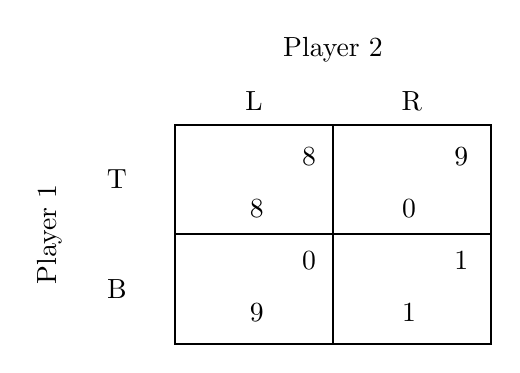
\begin{tikzpicture}
		\matrix[matrix of math nodes,
		every odd row/.style={align=right},every evenrow/.style={align=left},every node/.style={text width=1.5cm},row sep=0.2cm,column sep=0.2cm,ampersand replacement=\&] (m) {
			8\&9 \\
			8\&0 \\
			0 \&1 \\
			9 \&1\\
		};
		\draw (m.north east) rectangle (m.south west);
		\draw (m.north) -- (m.south);
		\draw (m.east) -- (m.west);
		
		% Player 1
		\coordinate (c) at ($(m.north west)!0.25!(m.south west)$);
		\coordinate (d) at ($(m.north west)!0.75!(m.south west)$);
		\node[left=2pt of c,text width=1cm]  {T};
		\node[left=2pt of d,text width=1cm]  {B};
		
		% Player 2
		\coordinate (a) at ($(m.north west)!0.25!(m.north east)$);
		\coordinate (b) at ($(m.north west)!0.75!(m.north east)$);
		\node[above=5pt of a,anchor=base] {L};
		\node[above=5pt of b,anchor=base] {R};
		
		\node[above=18pt of m.north] (firm b) {Player 2};
		\node[left=1.6cm of m.west,rotate=90,align=center,anchor=center] {Player 1};
		
		%\node[above=5pt of firm b]  {Payoff Matrix};
	\end{tikzpicture}
\end{figure}

\begin{parts}
	\part
	
	Payoff under (T,L):
	\begin{equation*}
		8 + \delta 8 + \delta^2 8 + \delta^3 8 + ... =  \frac{8}{1-\delta}
	\end{equation*}
	
	Payoff under deviation:
	\begin{equation*}
	9 + \delta + \delta^2 + \delta^3 ..... = 9 + \frac{\delta}{1-\delta}
	\end{equation*}
	
	In order for the strategy to be sustained we need:
	\begin{equation*}
		\frac{8}{1-\delta} \geq 9 + \frac{\delta}{1-\delta} \implies \delta \geq \frac{1}{8}
	\end{equation*}
	
	
\end{parts}

	\subsection*{Vertical Relationships (30 points)}
\question Suppose that there are two firms in a supply chain: a manufacturer who sells to a retailer. The timing is as follows:

\begin{enumerate}
	\item Manufacturer has a constant marginal cost $c=1$ and sets input price $w$ to maximize profit.
	\item Retailer buys input from manufacturer for price $w$. Retailer sets price $p$ to maximize profit with demand $D(p)= 8-p$.
\end{enumerate}
\begin{parts}
	\part
	Retailer's problem:
	\begin{gather*}
		MR = MC \implies 8 - 2q = w \\
		\implies q = \frac{8-w}{2}
	\end{gather*}
	
	Manufacturer's problem:
	\begin{gather*}
	\pi_m = (w-c)q = (w-1)(\frac{8-w}{2}) \\
	\frac{d \pi_m}{dw} = 0 : w = 3.5
	\end{gather*}
	
	Then,
	\begin{gather*}
	\pi_m = (3.5-1)2.25 = 5.625
	\pi_r = (8-3.5 - 2.25)2.25 = 5.0625 
	\end{gather*}
	
	\part Under vertical separation the retailer's price is too high due to double marginalization.
\end{parts}
\end{questions}

\end{document}